\chapter{Systemarkitektur}

Herunder vil systemet blive beskrevet overordnet med fokus på at skabe en forståelse for den store helhed. Ved at læse systemarkitekturen igennem vil/ burde læseren få en meget bedre forståelse for hvad systemet indebærer samt de store byggeblokke. For at forstå selve byggeelementerne samt hvordan de er sat sammen, skal læseren se i systemdesignet. Her vil mere implementeringsspecifikke detaljer være beskrevet. \\
For at give et overblik over systemet blev domænemodellen på Figur \ref{fig:system_domain} opsat. \\
\\

\textbf{Domænemodel}
\begin{figure}[H]
	\centering
	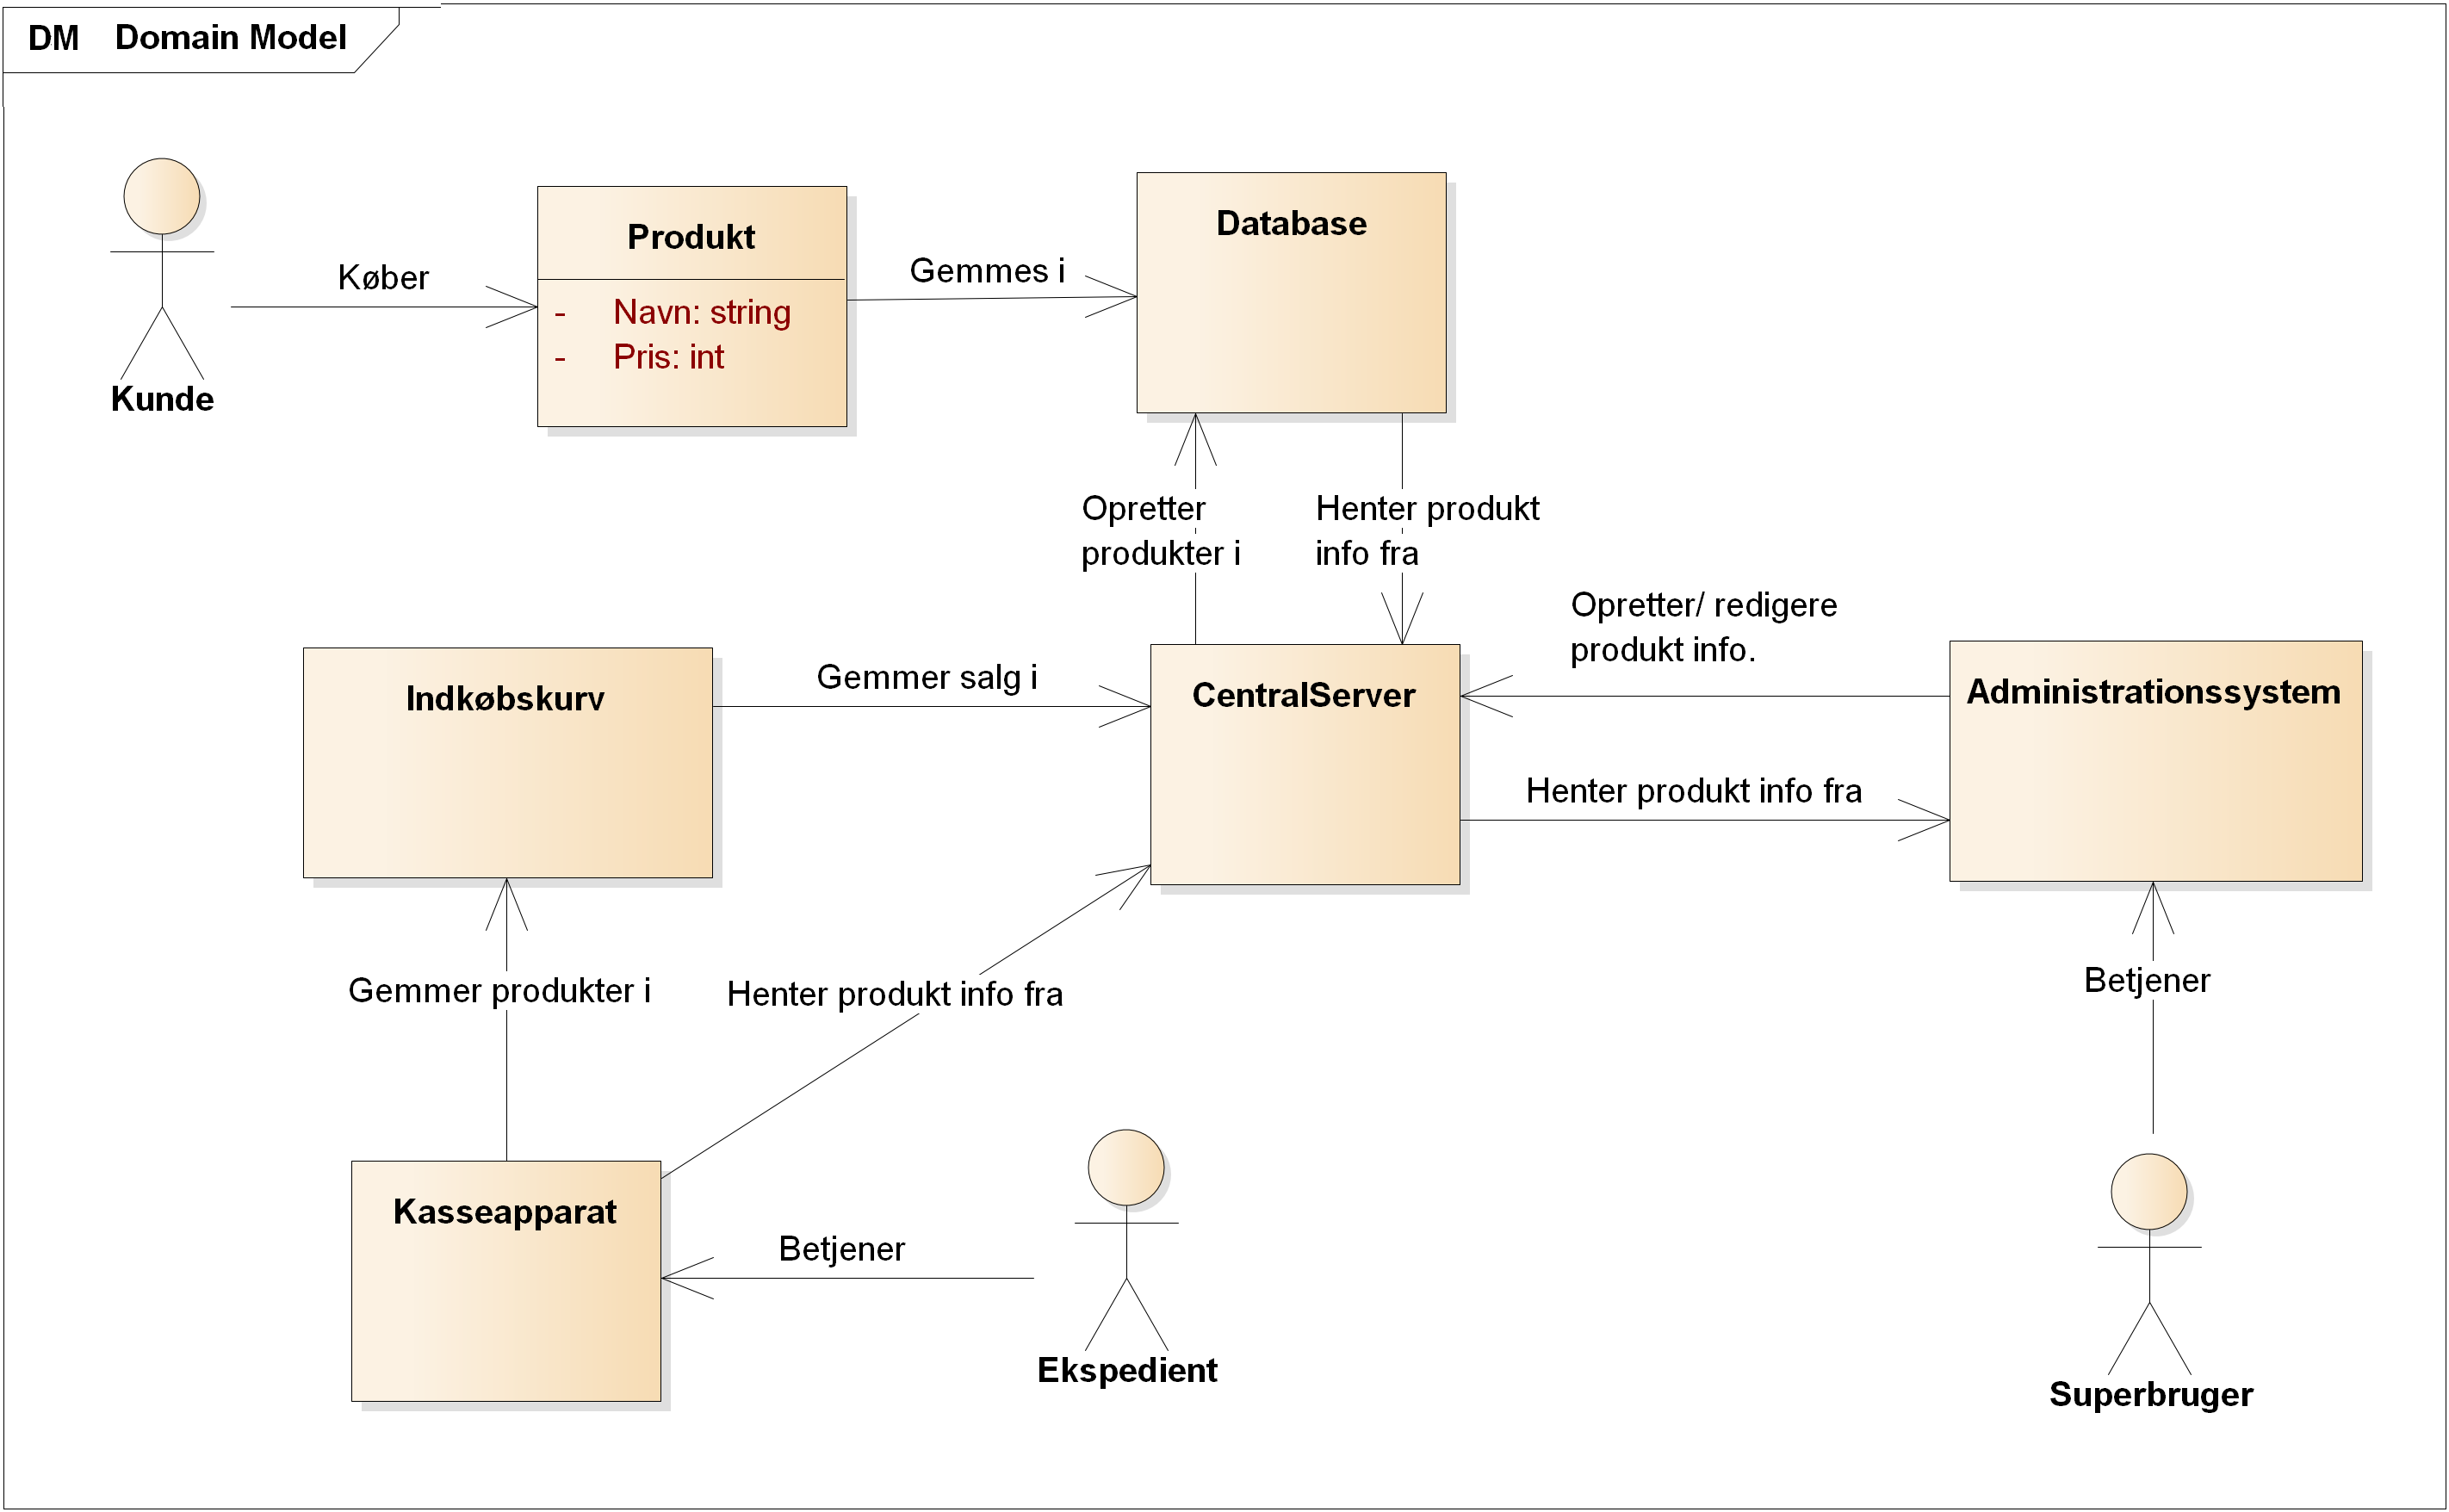
\includegraphics[scale=0.5]{Systemarkitektur/DomainModel}
	\caption{Domænemodel over systemet og dets overordnede dele}
	\label{fig:system_domain}
\end{figure}

Domænemodellen på figur \ref{fig:system_domain} viser systemets overordnede dele. En \textit{kunde} vil købe et \textit{produkt}. Dette \textit{produkt} ligger gemt i \textit{databasen}. \\ 
En \textit{ekspedient} betjener et \textit{kasseapparat}. Informationer om de \textit{produkter} der er til rådighed samt deres pris hentes fra \textit{CentralServeren}. Når en \textit{kunde} ønsker at købe et \textit{produkt}, så tilføjer \textit{ekspedienten} \textit{produktet}  til en \textit{indkøbskurv}. Når salget gennemføres gemmes salget i \textit{CentralServeren}. \\
Produkt informationer tilføjes, redigeres eller slettes af en \textit{superbruger} i \textit{administrationssystemet}. Disse ændringer afspejler \textit{CentralServeren} så i databasen.

\newpage

%\section{Use Case View}

\subsection{Oversigt over tråde}


%\newpage
\section{Logisk View}

\subsection{Oversigt over tråde}

\subsection{Arkitekturpakker}
Arkitekturpakkerne er en beskrivelse af de pakker der ses på diagrammet under oversigten, side \pageref{logical:oversigt}, figur \ref{logical:oversigt}. Beskrivelserne forklarer, hvad pakkens ansvar er og hvordan pakken kommunikerer med andre pakker i systemet.

\subsubsection{\gls{SL}}

\textbf{Ansvar}

\gls{SL} har i dette system ansvar for alt fælles logik, og bliver derfor tilgået af alle de tre delsystemer: \gls{KA}, \gls{CS} og \gls{AS}. \gls{SL} er et bibliotek indeholdende datamodeller, kommandoer og en protokol der sørger for at encode og decode disse kommandoer henholdsvis til og fra XML.
\subsubsection{\gls{DB}}

\textbf{Ansvar}

\gls{DB}n benyttes til at opbevare persistent data, herunder produkter, produktkategorier og køb. Det er udelukkende \gls{CS}, som interagerer med \gls{DB}.
\subsubsection{\gls{KA}}

\textbf{Ansvar} \\
Kasseapparatet er den del af systemet hvor produktkataloget bliver vist og benyttet til salg af produkter. Her laves kvitteringer og der bliver vist en liste/indkøbskurv med de produkter som en evt. kunde ønsker at købe. Produktkataloget bliver hentet ved en forespørgsel til Centralserver og kasseapparatet ved derved intet om oprettelse og redigering af de produkter som den fremviser. \\

\textbf{Sekvensdiagram}
\begin{figure}[H]
	\centering
	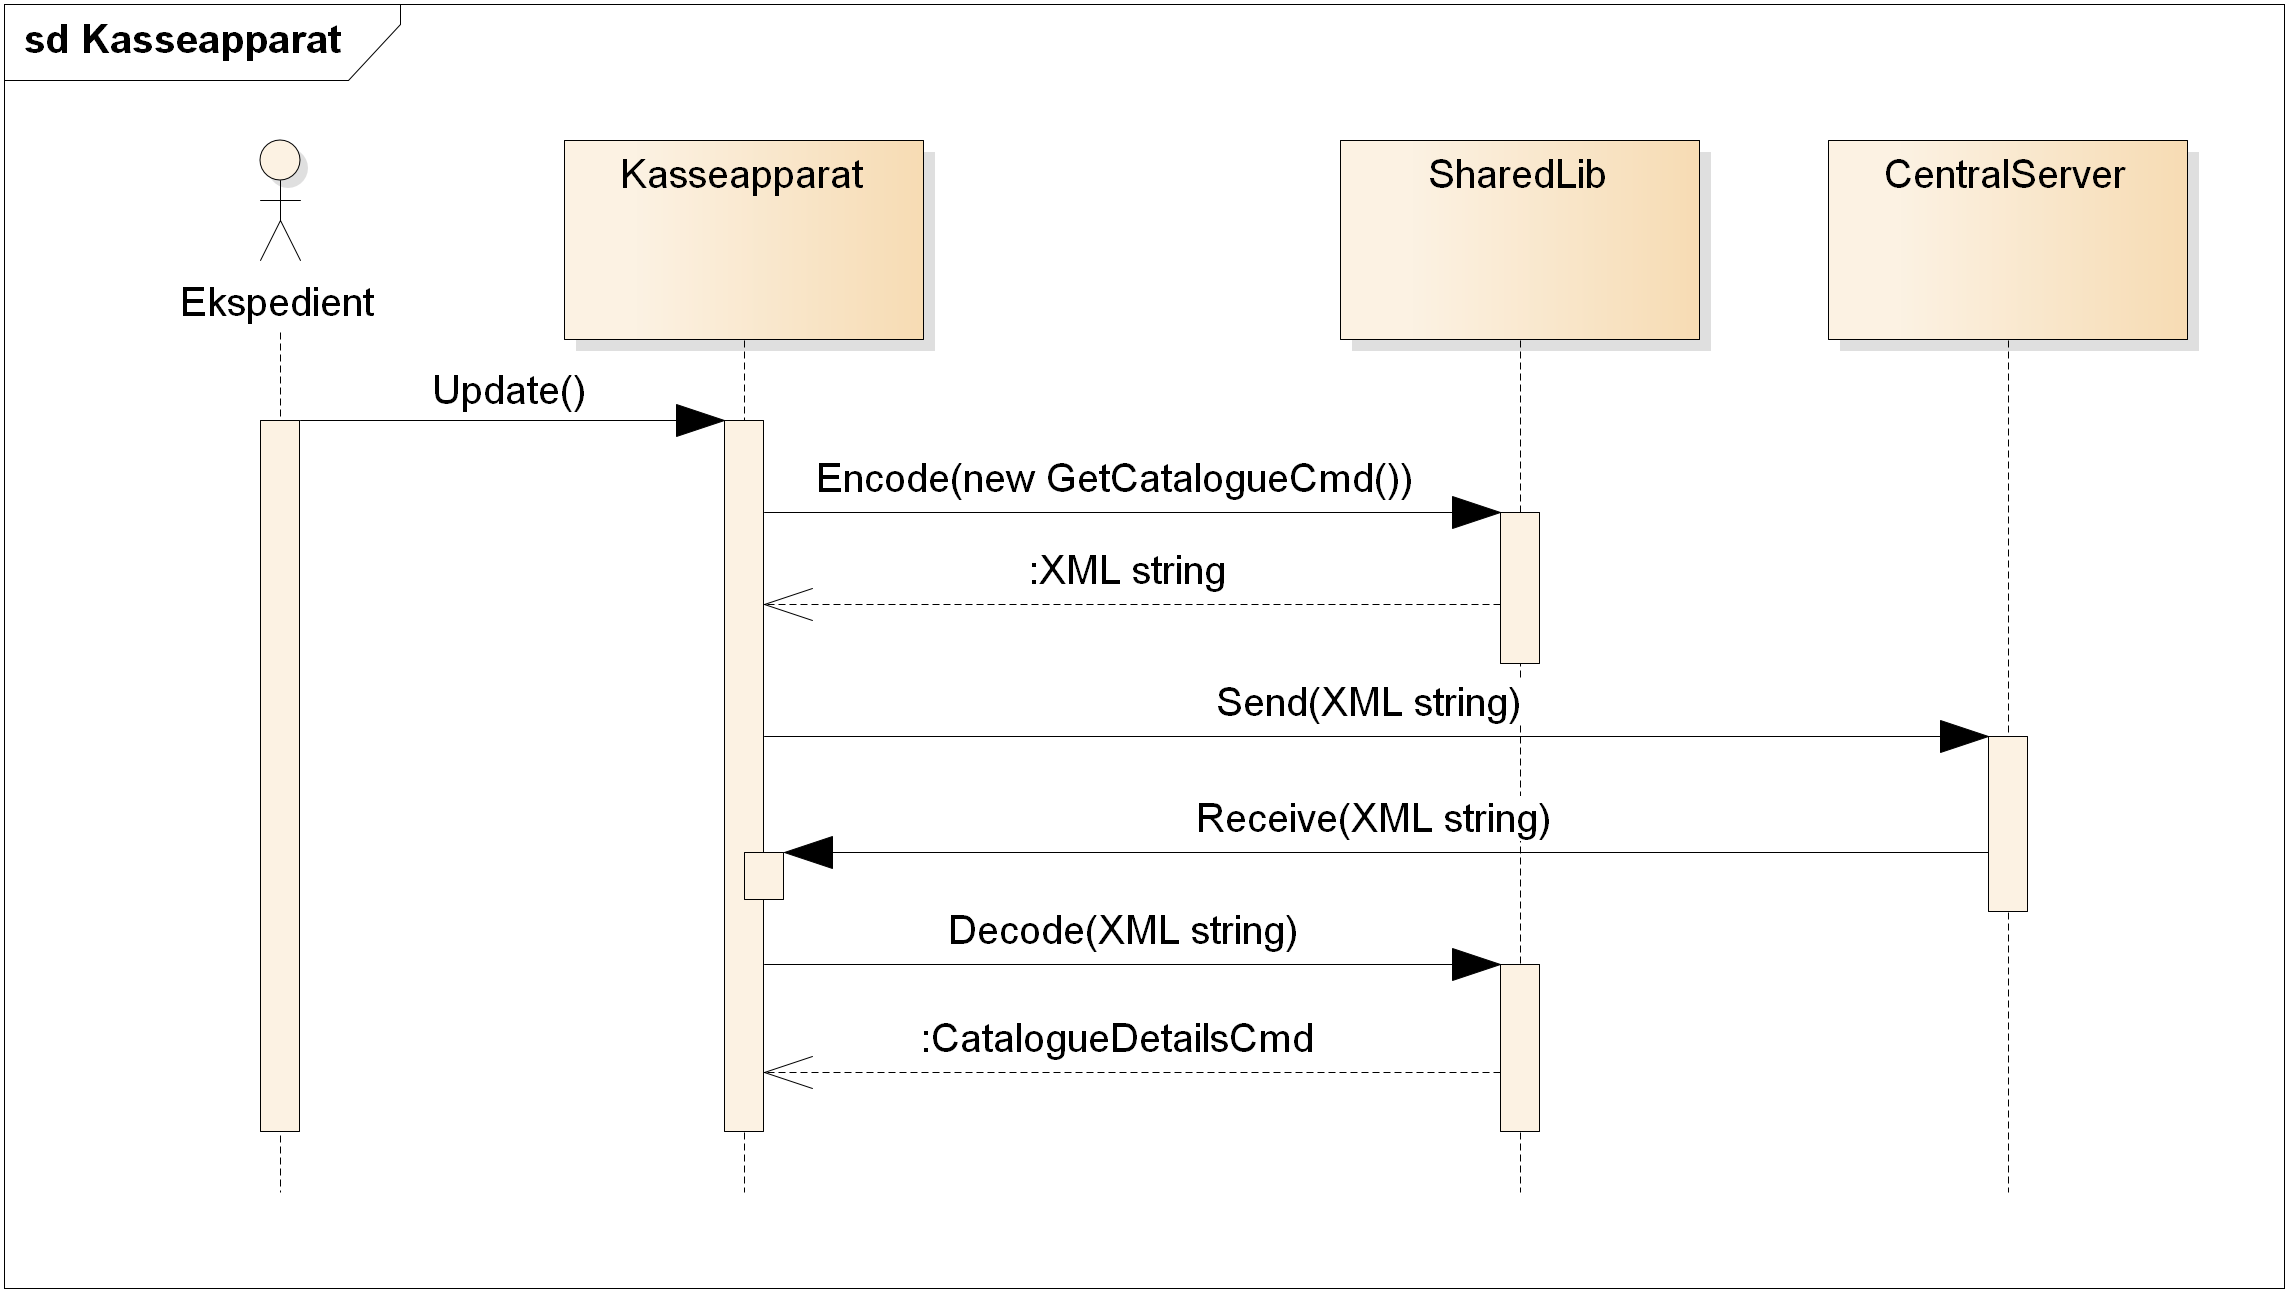
\includegraphics[scale=0.7]{Systemarkitektur/LogiskView/Kasseapparat-sekvensdiagram}
	\caption{Sekvensdiagram for kommunikation mellem \gls{KA} og andre pakker}
	\label{fig:logview_kasse_sekvensdiagram}
\end{figure}

Sekvensdiagrammet viser hvordan kasseapparatet kommunikerer med de andre pakker i systemet. Kasseaparatet kommunikerer udelukkende med Centralserver. Når kasseapparatet skal sende en besked til Centralserver bruger den SharedLib til at konvertere et kommandoobjekt til XML og sender herefter denne til Centralserveren. Centralserveren sender derefter en XML-besked tilbage som så derefter bliver omskrevet til et kommandoobjekt, igen ved brug af SharedLib.

\newpage

\subsubsection{CentralServer}

\textbf{Ansvar}\\
\gls{CS} har til ansvar at få videreformidlet kommandoer og fungerer på denne måde som mellemled imellem pakkerne. Derudover har \gls{CS} også ansvar for at indsætte og hente data fra databasen.\\

\textbf{Sekvensdiagram}

\begin{figure}[H]
    \centering
    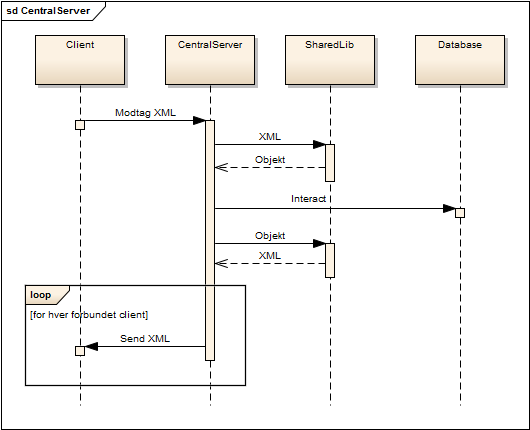
\includegraphics[width=0.8\textwidth]{Systemarkitektur/LogiskView/CentralServer.PNG}
    \caption{Sekvensdiagram for kommunikationen mellem \gls{CS} og andre pakker.}
    \label{fig:cssekv}
\end{figure}

På figur \ref{fig:cssekv} ses hvordan \gls{CS}, når den modtager XML, benytter \gls{SL} til at konvertere det modtagede XML til et højniveau kommando-objekt, som \gls{CS} herefter kan agere på. Det enten værende indsættelse/sletning af data i databasen eller andet. Til sidst vil \gls{CS} igen benytte \gls{SL} til at konverete et højniveau svar om til XML, som sendes ud til alle tilstedeværende klienter.\\\\

Dette er det typiske sekvens af kommunikation mellem klient og server, men det er ikke noget krav, at \gls{CS} agerer på den modtagede besked, eller for den sags skyld svarer tilbage til klienten.
\subsubsection{\gls{AS}}
\textbf{Ansvar}\\
\gls{AS} er den del af systemet, hvor produktkataloget bliver redigeret. Dette indebærer oprettelse, sletning og ændring af produkter, såvel som produktkategorier. \gls{AS} bliver betjent af \gls{SB}, se aktørkontekst diagram, figur \ref{fig:aktcont} side \pageref{fig:aktcont}.\\

\textbf{Sekvensdiagram}
\begin{figure}[H]
	\centering
	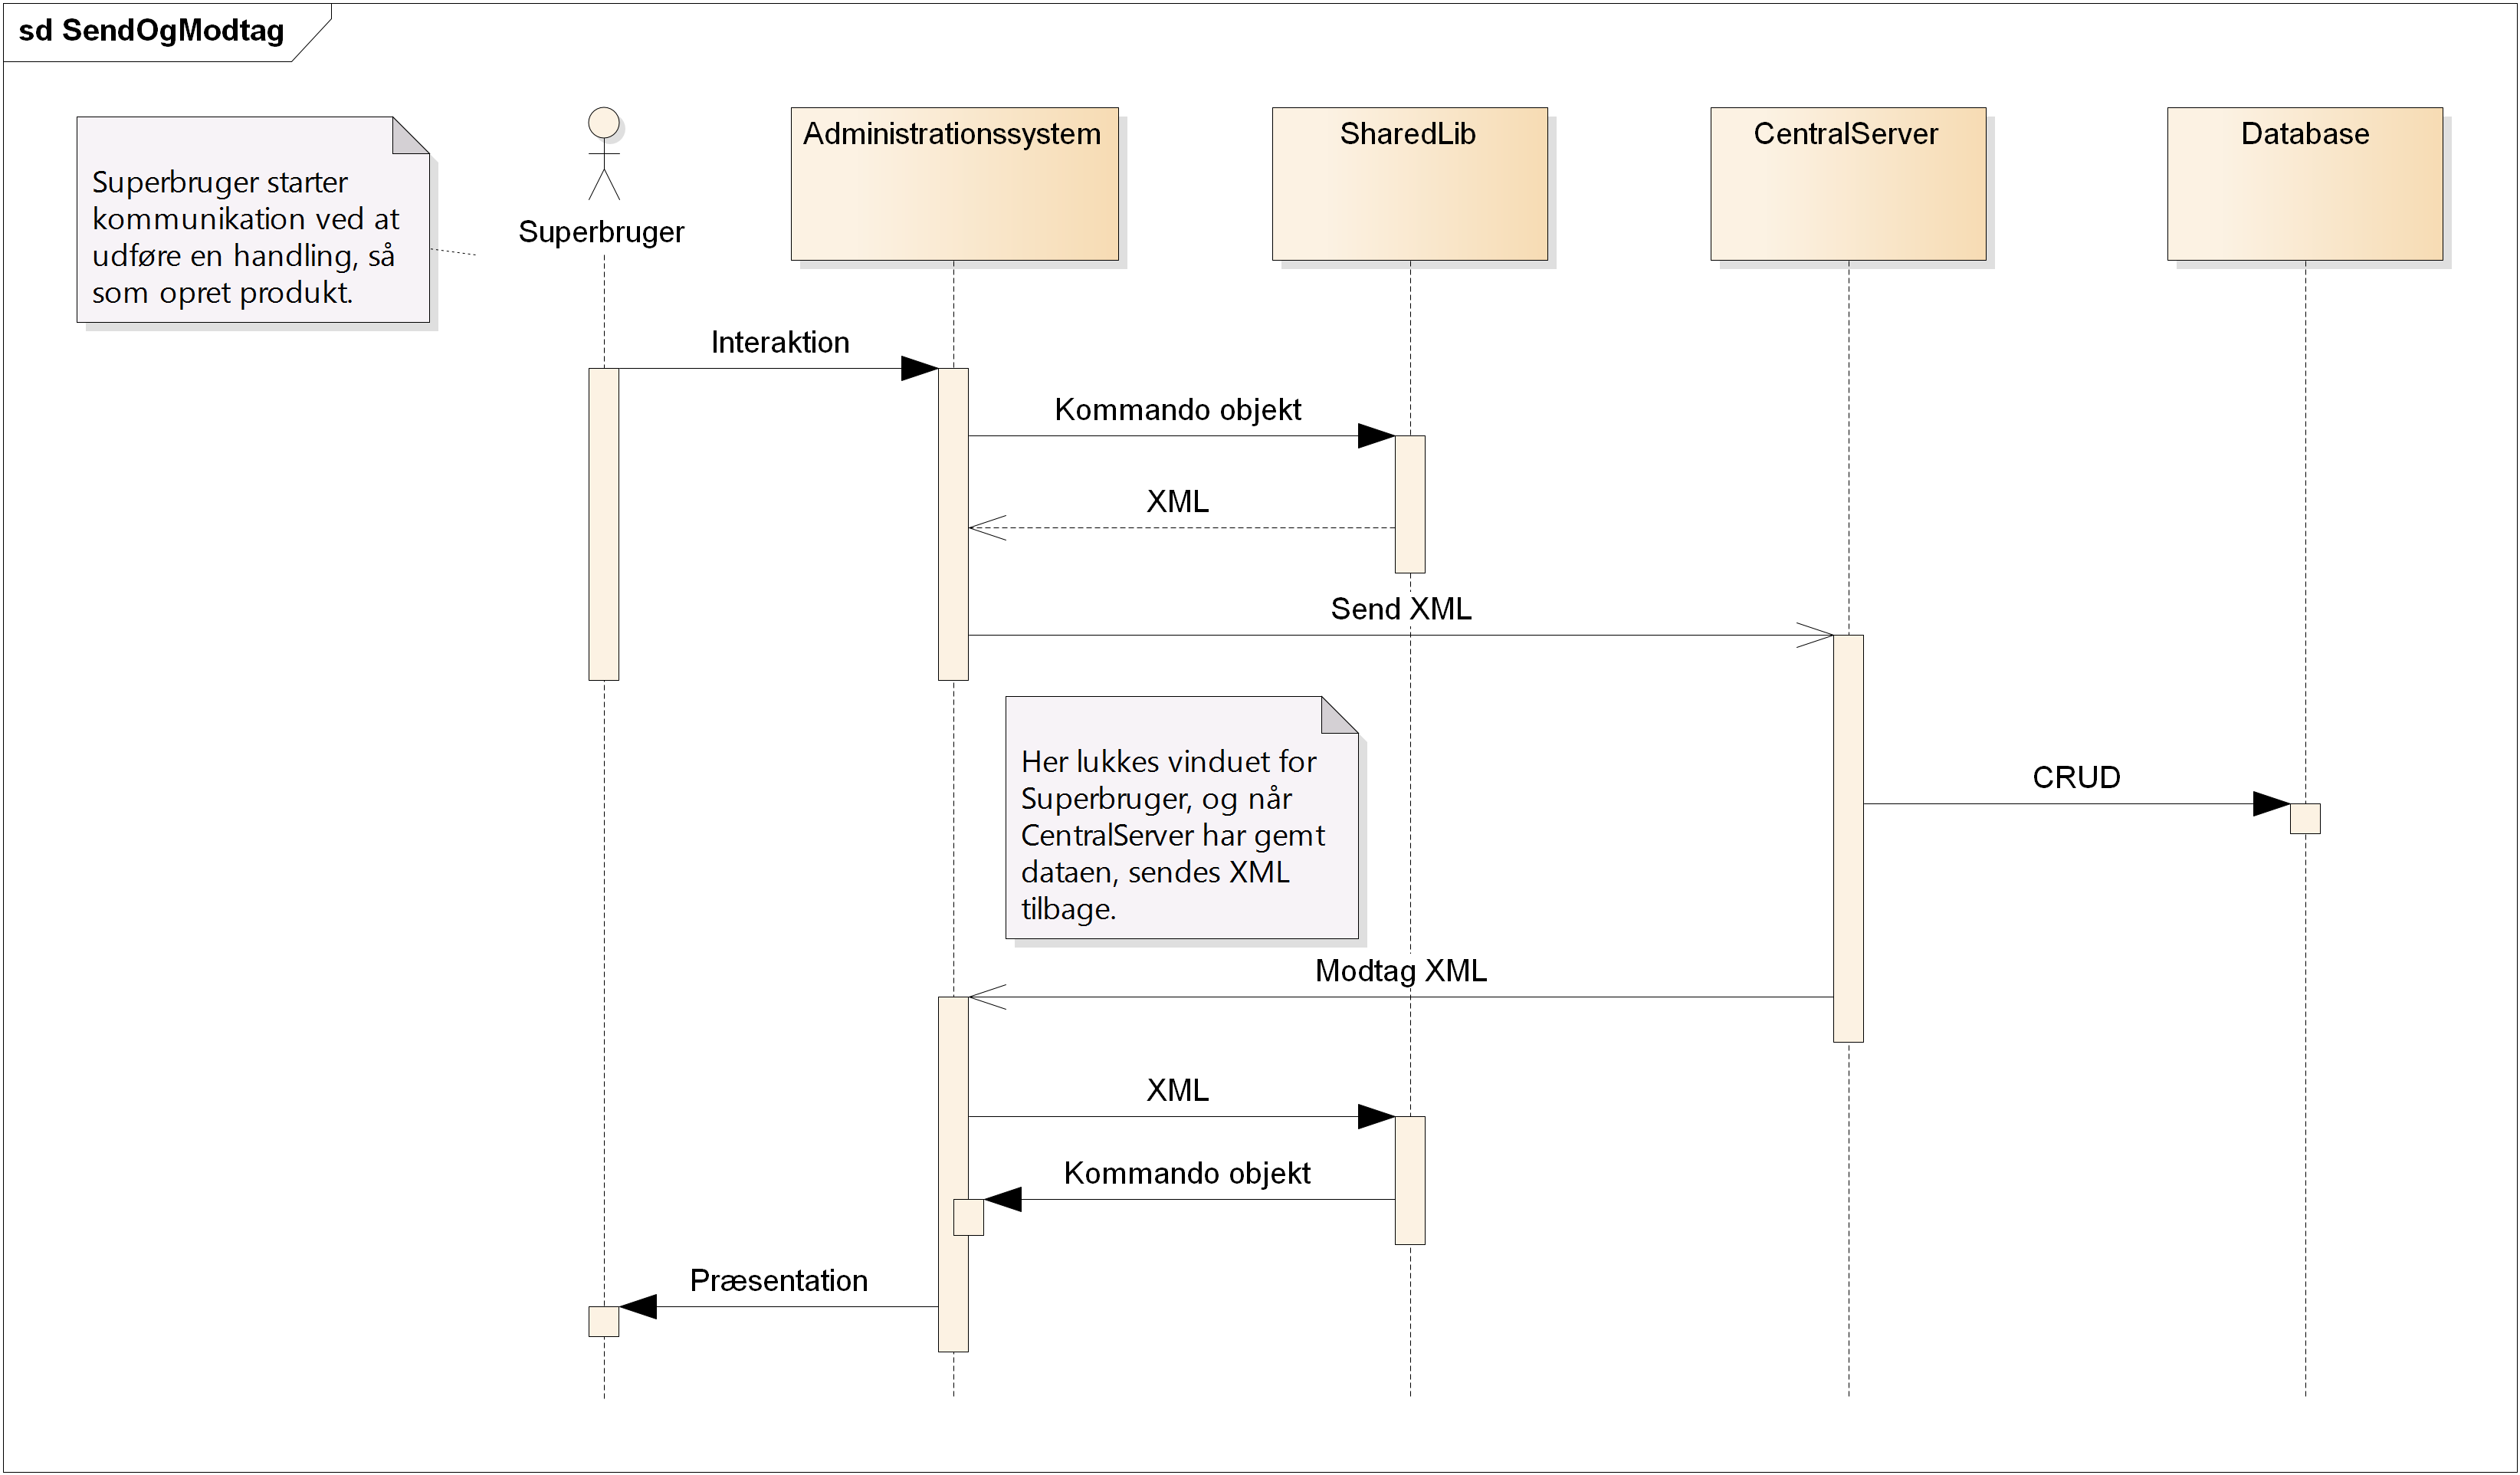
\includegraphics[width=\textwidth]{Systemarkitektur/LogiskView/Administrationssystem-sekvensdiagram}
	\caption{Sekvensdiagram for kommunikation mellem \gls{AS} og andre pakker}
	\label{fig:logview_admin_sekvensdiagram}
\end{figure}

Sekvensdiagrammet på figur \ref{fig:logview_admin_sekvensdiagram} viser den kommunikation der foregår mellem \gls{AS}et og de andre pakker i systemet. \gls{AS}et kommunikerer udelukkende med \gls{CS}, mens \gls{SL} bliver brugt til at encode og decode XML strenge der sendes og modtages fra \gls{CS}. Sekvensdiagrammet (figur \ref{fig:logview_admin_sekvensdiagram}) viser udelukkende interfacet mellem pakkerne. Uddybende forklaring af \gls{AS} pakken kan findes under dens designafsnit, se afsnit \ref{section:design_admin}.


\subsection{Use Case realiseringer}

\textbf{Use Case 1 - Gennemfør salg}

Disse Use Cases beskriver følgende funktionalitet:
\begin{itemize}
	\item Gennemfør salg
	\item Returner vare
\end{itemize}
Funktionaliteten til disse Use Cases ligner hinanden. Når \gls{Eks} har udført de nødvendige
handlinger i \gls{KA} \gls{GUI} og trykker på knappen til at afslutte handel, så bliver der sendt data til \gls{CS}.

Når ekspedienten har gennemført et salg/retur i \gls{KA} så vil følgende
handlinger blive udført i systemet:
\begin{itemize}
	\item \gls{KA} opretter det korrekte kommando objekt, via \gls{SL}, med informationerne for handlen
	\item \gls{KA} bruger \gls{SL} til at konvertere kommando objektet til en XML streng
	\item XML strengen sendes til \gls{CS}
	\item \gls{CS} modtager strengen og konverterer den tilbage til den oprindelige kommando, igen ved hjælp af \gls{SL}
	\item \gls{CS} udfører de nødvendige handlinger på \gls{DB}
\end{itemize}

\begin{figure}[H]
	\centering
	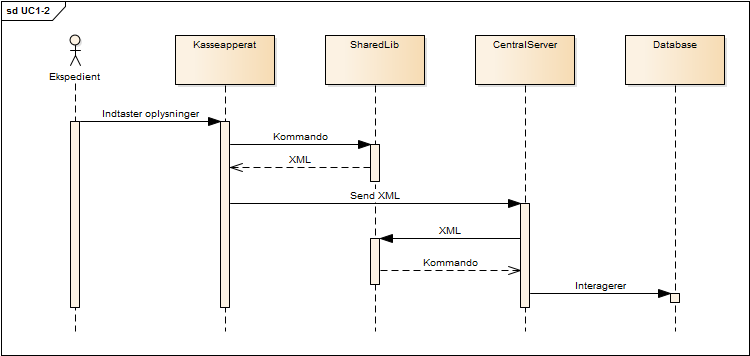
\includegraphics[width=0.8\textwidth]{Systemarkitektur/LogiskView/Realiseringer/Images/UC12.png}
	\caption{Sekvensdiagram for realisering af Use Cases 1 og 2}
	\label{fig:uc38sq}
\end{figure}


\textbf{Use Cases 3-8}\\
Disse Use Cases beskriver følgende funktionalitet:
\begin{itemize}
	\item Opret produkt
	\item Rediger produkt
	\item Slet produkt
	\item Opret kategori
	\item Rediger kategori
	\item Slet kategori
\end{itemize}
Funktionaliteten til disse Use Cases ligner hinanden. Når gls{SB} har udført de nødvendige handlinger i \gls{AS}ets grafiske brugerflade og trykker på knappen til at godkende handlingen, så bliver der sendt data til \gls{CS} og efterfølgende modtaget data fra \gls{CS}.

Når \gls{SB} har modificeret et produkt eller en kategori i \gls{AS}, så vil følgende handlinger blive udført i systemet:
\begin{itemize}
	\item \gls{AS} opretter et kommando objekt af den rette type, med informationerne for handlingen.
	\item \gls{AS} bruger \gls{SL} til at konvertere kommando objektet til en XML streng.
	\item XML strengen sendes til \gls{CS}.
	\item \gls{CS} modtager strengen og konverterer den tilbage til den oprindelige kommando, igen ved hjælp af \gls{SL}.
	\item \gls{CS} udfører de nødvendige handlinger på \gls{DB}.
	\item \gls{CS} opretter et kommando objekt med det rette svar (f.eks. ProductCreated efter den har oprettet et produkt).
	\item \gls{CS} konverterer kommandoen til en XML streng ved hjælp af \gls{SL}.
	\item \gls{CS} sender XML strengen til alle de klienter der er forbundet til \gls{CS}.
\end{itemize}

Funktionaliteten for Use Casene er beskrevet med et sekvensdiagram, som vises på figur \ref{fig:uc38sq}.

\begin{figure}[H]
    \centering
    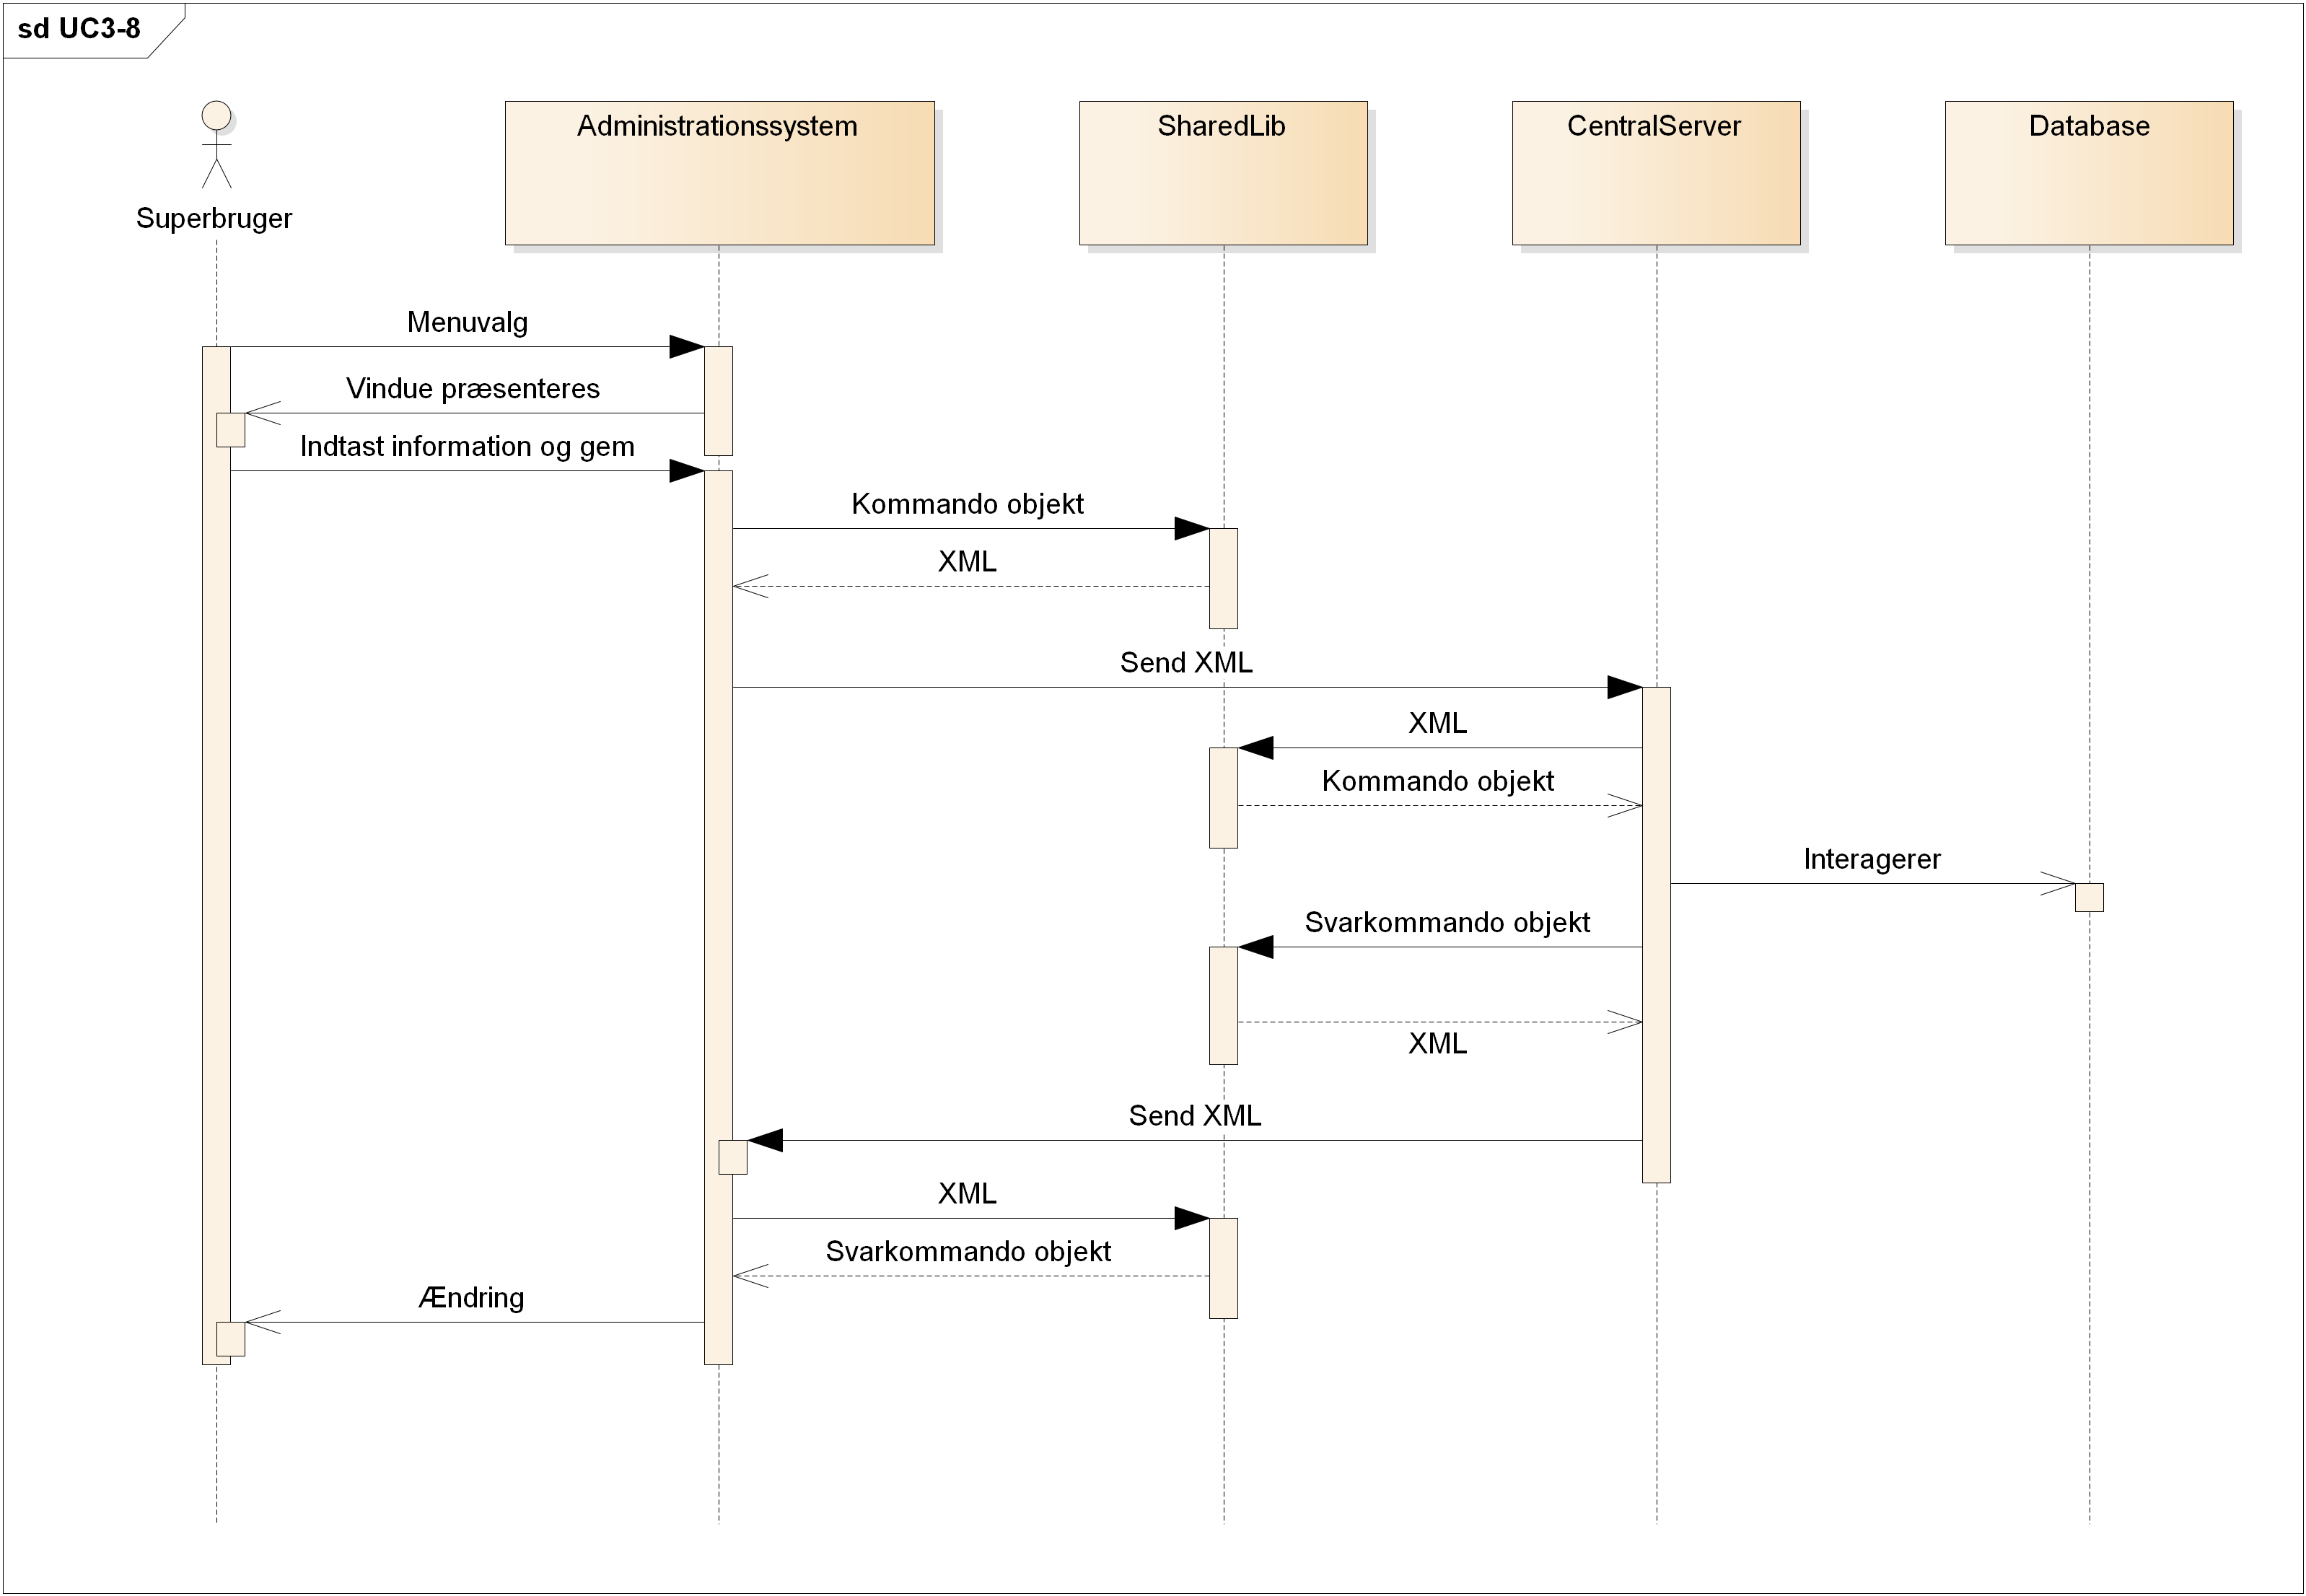
\includegraphics[width=0.8\textwidth]{Systemarkitektur/LogiskView/Realiseringer/Images/UC38.png}
    \caption{Sekvensdiagram for realisering af Use Cases 3 til 8.}
    \label{fig:uc38sq}
\end{figure}

Når CentralServer svarer, er der på sekvensdiagrammet (figur \ref{fig:uc38sq}) afbilledet, at den blot svarer til Administrationssystemet. I realiteten broadcaster den svaret til alle klienter der er forbundet. Dette er dog ikke vigtigt for forståelsen af kommunikationen i disse Use Cases.
\newpage
%\section{Proces/Task View}

\subsection{Oversigt over tråde}


%\newpage
\section{Physical View}

\subsection{Oversigt over tråde}

\subsection{Node Beskrivelser}

\subsubsection{Kasseapparat}
\gls{KA} kommunikerer med \gls{CS} gennem en TCP/IP forbindelse. Forbindelsen benyttes til at hente produktkataloget samt at registrere køb.

\subsubsection{Administrationssystem}
\gls{AS} kommunikerer med \gls{CS} gennem en TCP/IP forbindelse. Forbindelsen benyttes til at hente produktkataloget samt at oprette, redigere og slette produkter og produktkategorier.

\subsubsection{CentralServer}
\gls{CS} stiller en server til rådighed, som \gls{KA} og \gls{AS} kan forbinde til (beskrevet ovenfor). \gls{CS} foretager også alt den nødvendige interaktion med Database.

\subsubsection{Database}
Interageres med af \gls{CS}.
\newpage
\section{Development View}

\subsection{Oversigt over tråde}

\subsection{Komponentbeskrivelser}

\subsubsection{Administrationssytstem}
Denne bruger \gls{SL} i samtlige lag. Dette indebærer visning modeller i brugergrænsefladen, samt benyttelse af protokoller til at sende og modtage data.

\subsubsection{CentralServer}
Denne benytter \gls{SL} til protokoller og modeller.

\subsubsection{Kasseapparatet}
Benytter ligesom \gls{AS}, \gls{SL} i dets grafiske lag samt business logic lag. Igen bruges der modeller og protokoller så alle er enige om disse.

\subsubsection{SharedLib}
Denne er en fælles afhængighed for alle systemets komponenter. \gls{SL} indeholder fælles modeller (Produkter, produktkategorier), kommandoer der skal sendes til og fra \gls{CS} og protokol til at encode og decode kommandoerne.
